\documentclass[a4paper,
               %boxit,
               %titlepage,   % separate title page
               %refpage      % separate references
              ]{jacow}

\makeatletter%                           % test for XeTeX where the sequence is by default eps-> pdf, jpg, png, pdf, ...
\ifboolexpr{bool{xetex}}                 % and the JACoW template provides JACpic2v3.eps and JACpic2v3.jpg which might generates errors
 {\renewcommand{\Gin@extensions}{.pdf,%
                    .png,.jpg,.bmp,.pict,.tif,.psd,.mac,.sga,.tga,.gif,%
                    .eps,.ps,%
                    }}{}
\makeatother

\ifboolexpr{bool{xetex} or bool{luatex}} % test for XeTeX/LuaTeX
 {}                                      % input encoding is utf8 by default
 {\usepackage[utf8]{inputenc}}           % switch to utf8

\usepackage[USenglish]{babel}
\usepackage{balance}


\ifboolexpr{bool{jacowbiblatex}}%        % if BibLaTeX is used
 {%
  \addbibresource{jacow-test.bib}
  \addbibresource{biblatex-examples.bib}
 }{}

\newcommand\SEC[1]{\textbf{\uppercase{#1}}}

%%
%%   Lengths for the spaces in the title
%%   \setlength\titleblockstartskip{..}  %before title, default 3pt
%%   \setlength\titleblockmiddleskip{..} %between title + author, default 1em
%%   \setlength\titleblockendskip{..}    %afterauthor, default 1em

%\copyrightspace %default 1cm. arbitrary size with e.g. \copyrightspace[2cm]

% testing to fill the copyright space
%\usepackage{eso-pic}
%\AddToShipoutPictureFG*{\AtTextLowerLeft{\textcolor{red}{COPYRIGHTSPACE}}}

\usepackage{url}            % \url command for decent line breaks in urls

\begin{document}

\title{Cern Open Hardware Experience: Upgrading the Diamond Fast Archiver}

\author{I.S. Uzun and M. Abbott, Diamond Light Source, Oxfordshire (UK)}

\maketitle

%
\begin{abstract}
Diamond Light Source developed and integrated the Fast Archiver~\cite{ARCHIVER} into its Fast Orbit Feedback (FOFB) communication network in 2009. It enabled synchronous capture and archive of the entire position data in real-time from all Electron Beam Position Monitors (BPMs) and X-Ray BPMs. The FA Archiver solution has also been adopted by SOLEIL and ESRF. However, the obsolescence of the existing PCI Express (PCIe) based FPGA board from Xilinx and continuing interest from community forced us to look for a new hardware platform while keeping the back compatibility with the existing Linux kernel driver and application software. This paper reports our experience with using the PCIe SPEC card from CERN Open Hardware initiative as the new FA Archiver platform. Implementation of the SPEC-based FA Archiver has been successfully completed and recently deployed at ALBA in Spain.
\end{abstract}

\section{Introduction}
The Diamond FOFB system is operating successfully and achieving the required level of suppression of beam disturbances since 2007~\cite{FOFB}. The system architecture for the FOFB for a single Storage Ring (SR) cell is shown in Fig~\ref{FOFB}. Diamond SR consists of 24 cells, and overall FOFB architecture consists of: 

\begin{itemize}
\setlength\itemsep{0em}
\item 172 Electronic Beam Position Monitors (BPMs) located around the storage ring.
\item 24 VME-based processors, each populated with a PMC receiver, running the feedback algorithm.
\item Power supply controller units for 168 slow corrector magnets.
\item Communication network to distribute the beam position values.
\end{itemize}

\begin{figure}[b!]
   \centering
   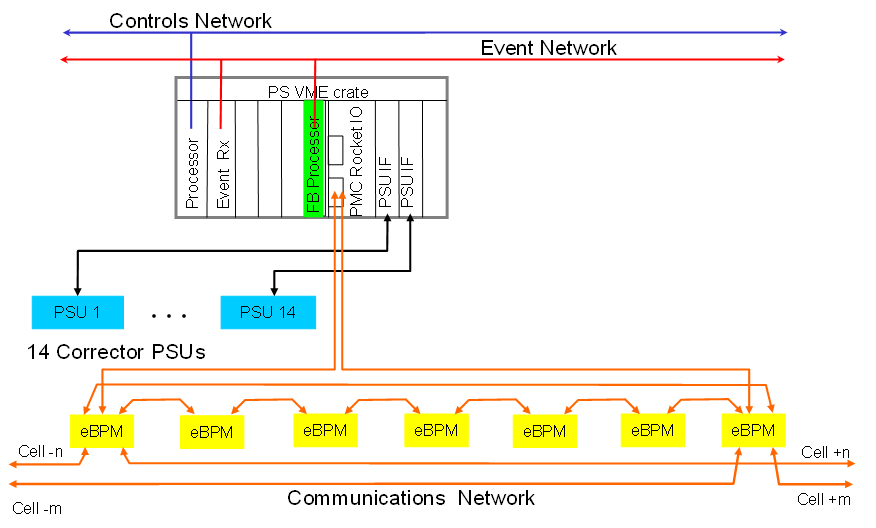
\includegraphics[width=80mm]{img/WEPGF089f1}
   \caption{FOFB architecture for single SR Cell. It is repeated for each 24 cells in Diamond SR.}
   \label{FOFB}
\end{figure}

BPMs are used for electron beam diagnostics. In the BPM FPGA the sampled button intensities are converted to X,Y positions and reduced by decimation and filtering to machine revolution frequency (534 kHz) and then to the “Fast Acquisition” (FA) data rate of 10 kHz and the “Slow Acquisition” rate of 10 Hz for EPICS clients. The FA data is broadcast by Diamond Communication Controller IP (DCC)~\cite{DCC} on the FPGA through a dedicated communication network, which makes this data stream simultaneously available to all PMC receiver nodes on VME processors for fast feedback processing. 

Following the successful operation of FOFB system, a need for recording longer periods of synchronous position data from all nodes on the communication network (the whole orbit) at FA data rate was identified. The DCC IP and dedicated communication network enabled us to additional nodes with little or no impact on the operation of the FOFB; and the FA Archiver is one such node implemented on a PCIe hardware~\cite{ARCHIVER}.

Two FA Archiver nodes have been running at Diamond, one for Booster and one for Storage Ring since 2009, giving us access to records of up to two weeks of position data across the both rings. We have been using this data for:

\begin{itemize}
\setlength\itemsep{0em}
\item Identification and detailed investigation of any orbit events that happened in the recent past.
\item Correlation of orbit events with other measurements by adding X-ray BPMs and RF cavity voltage readings to the FA network.
\item Model analysis of orbit motion over longer periods for the optimisation of the fast orbit feedback.
\end{itemize}

FA Archiver interface was implemented on a commercial Xilinx ML555 PCIe FPGA~\cite{ML555} board as a cost-effective solution so that we could focus our efforts on firmware development and software integration. Following its successful commissioning at Diamond, SOLEIL and ESRF integrated FA Archiver as part of their fast feedback system. This was possible since both facilities built their FOFB data distribution network using DCC giving them the protocol compatibility required.

\begin{figure*}[t!]
   \centering
   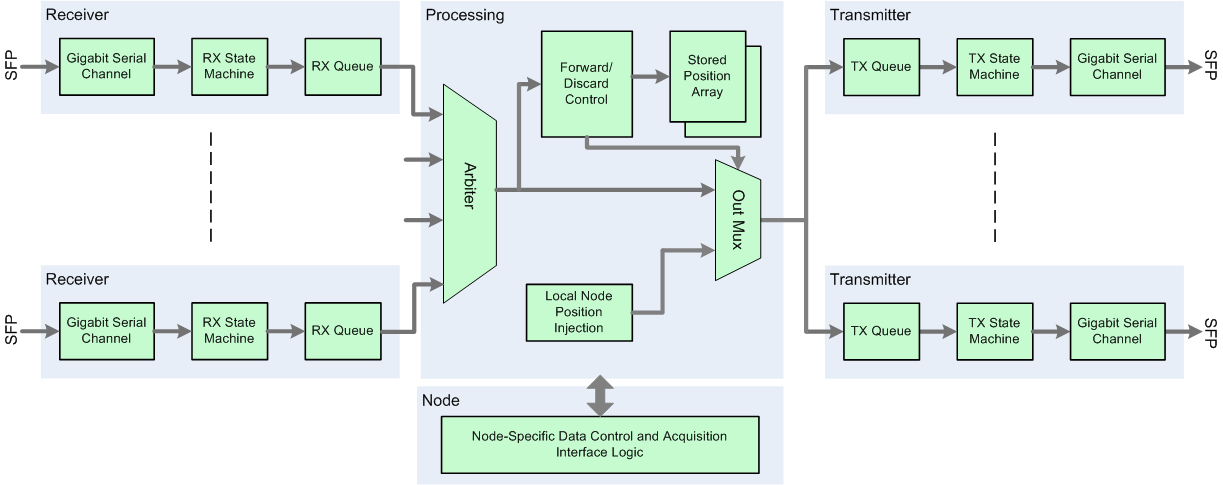
\includegraphics[width=140mm]{img/WEPGF089f3}
   \caption{Major building blocks of DCC design.}
   \label{DCC}
\end{figure*}

Recent interest from ALBA as the latest user of DCC, and Brazilian Light Source (LNLS) for evaluation purposes brought the obsolescence of the ML555 platform to our attention. In order to support the community, we took on an upgrade project targeting implementation of FA Archiver on a modern platform with longer term support and availability. Following evaluation of commercially available products and in-house built possibilities, we have decided that SPEC card from CERN Open Hardware initiative would be the best candidate due to its wide use in the accelerator community for various projects and openness of the design sources.

\section{Diamond Communication Controller}

To realise the required data transfer (BPMs to computation nodes) at a 10 kHz update rate, DCC IP was designed and implemented in VHDL. The IP uses Multi-gigabit Serial Transceivers (MGTs) on the FPGA achieving communication rate of 2.12 Gbps for Diamond.

DCC utilises a data-forwarding protocol whereby each node forwards its own data, plus each piece of incoming data once. The data is encapsulated in a low-overhead packet including CRC. The architectural block diagram of the DCC is shown in Fig~\ref{DCC}. The IP design consists of three main blocks:

\begin{itemize}
\setlength\itemsep{0em}
\item Receiver block implements up to 4 input channels, and is responsible for de-serialising, decoding, CRC checking and queuing the incoming packets.
\item Data Processing (Store, Analyse and Forward) keeps tracks of incoming packets from each node on the communication network, and transmits a specific node's packet only once in a given timeframe. This approach prevents flooding the communication network. It also stores received values for feedback or archiving purposes.
\item Transmitter block implements output queues for each channel. It is responsible for adding CRC, encapsulating and encoding position data for transmission through the serial links.
\end{itemize}

A dedicated fibre network between BPMs was chosen as a cost effective method of achieving low-latency communication. The BPMs have four SFP multi-gigabit serial transceivers, the 24 storage ring cells are wired in a torus network with single-mode fibre while copper patch cables are used intra-cell. The DCC network topology is structured as a 2D torus, with one computation node per SR cell, and gives a degree of resilience to failure of single or combinations of BPMs or links. The communication network structure is shown in Fig.~\ref{NETWORK}.

\begin{figure}[b!]
   \centering
   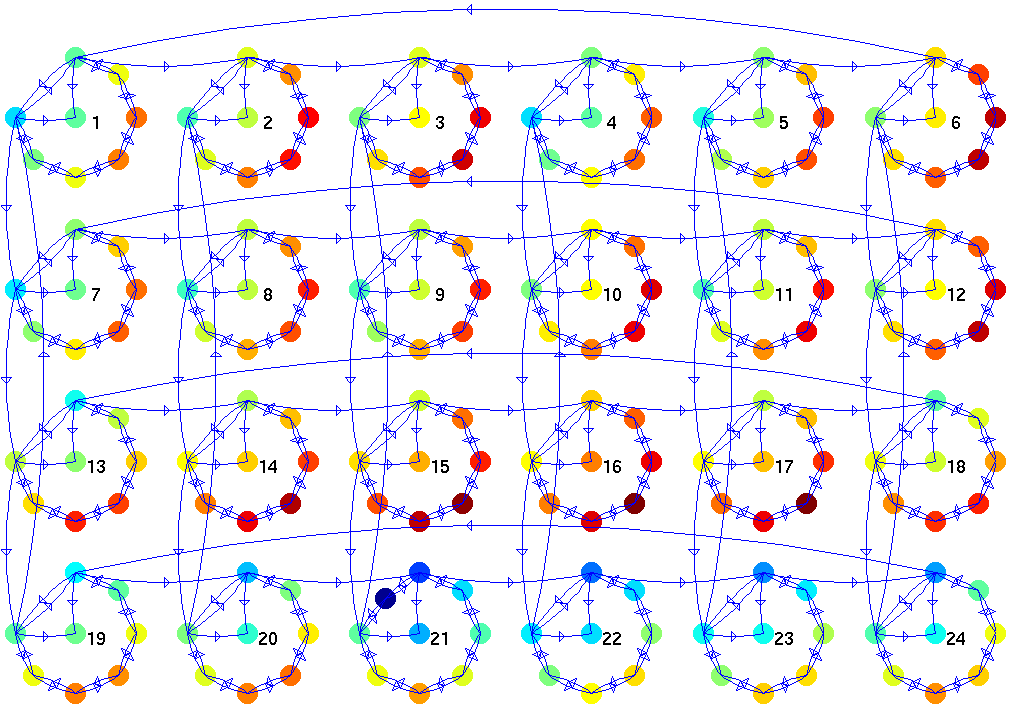
\includegraphics[width=70mm]{img/WEPGF089f2}
   \caption{Communication network topology, with each circle being one cell consisting of seven BPMs, and a PMC receiver in the centre. The coloring represents total distribution time for each node.}
   \label{NETWORK}
\end{figure}

\section{Diamond FA Archiver}

The design of the DCC and communication network makes it easy to add new nodes to the network, both as contributors and as passive listeners. The FA archiver acts as a passive listener storing the data stream in a 30TB ring buffer. The stored data is then available to clients via a set of software tools.

Implementation of FA archiver interface requires a PCIe form factor hardware platform with following on-board resources:

\begin{itemize}
\setlength\itemsep{0em}
\item Minimum 1-lane of PCIe bus interface. This could be either through dedicated IPs blocks on an FPGA device or a bridge chip external to the FPGA.
\item At least 1 MGT on the FPGA for DCC implementation.
\item On-board SFP connector(s) for physical connection to the communication network.
\item Clocking resources required for PCIe, DMA data transfer and DCC FPGA logic.
\end{itemize}

The FPGA design for the FA Archiver is shown in Fig~\ref{SNIFFER}. It integrates the DCC into a bus master PCIe architecture on the ML555 FPGA board. The design consists of target logic, DMA initiator logic, status/control registers and the Virtex-5 endpoint core for PCIe. Target logic is responsible for capturing single doubleword memory write and memory read PCIe Transaction Layer Packets (TLPs) for control and status register access. The DMA initiator logic generates memory write TLPs to transfer 4K byte frame data from the DCC core to the host’s system memory through PCIe endpoint.

\begin{figure}[t!]
   \centering
   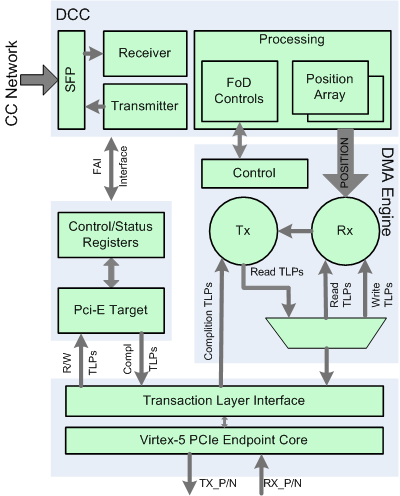
\includegraphics[width=70mm]{img/WEPGF089f4}
   \caption{Architecture of the FA Archiver FPGA design on ML555 board. The design directly interfaces to PCIe physical connector.}
   \label{SNIFFER}
\end{figure}

\section{CERN Open Source Hardware}
Open source hardware (OHW) is hardware whose design is made publicly available so that anyone can study, modify, distribute, make, and sell the design or hardware based on that design~\cite{OHW}. Open hardware has in recent years established itself as a very effective way for CERN to make electronics designs and in particular printed circuit board layouts, accessible to anyone, while also  facilitating collaboration and design re-use. It is creating an impact on  many levels, from companies producing and selling products based on  hardware designed at CERN, to new projects being released under the CERN Open Hardware Licence (OHL)~\cite{OHL}. Today the open hardware community includes large research institutes, universities, individual enthusiasts and companies. Many of the companies are actively involved in the  entire process from design to production, delivering services and consultancy and even making their own products available under open licences.

\subsection{Open Hardware Repository}
Recognizing the benefits that an open source philosophy could provide to hardware development and dissemination, CERN created the Open Hardware Repository(OHR) in 2009. It is a place on the web for electronics designers at experimental physics facilities to collaborate on open hardware designs. Technical specifications, research documents, CAD drawings and HDL code relating to projects are available for download from the OHR version control system. The Open Hardware Repository currently hosts more than 100 projects, ranging from small projects with a few collaborators to bigger projects with multiple contributors from both industry and academia. A dozen companies are actively involved in projects in the OHR and some of them are producing the physical hardware for CERN and other customers.

One of the prominent projects within OHW framework is the Simple PCIe FMC carrier (SPEC) card developed by CERN, as shown in Fig~\ref{SPEC}. SPEC is a data-acquisition card that can be plugged in to a PC, allowing the use of different FMCs, such as a digital input/output module, a time-to-digital converter and a fine delay module. The SPEC card was designed with the White Rabbit (WR) timing project in-mind and is the most widely-sold card offering WR support for synchronization. Several companies sell the card and are involved in its development. SPEC cards have found their way to many scientific applications, such as fusion energy, tracking of space debris and control systems for accelerator complexes.

\begin{figure}[t!]
   \centering
   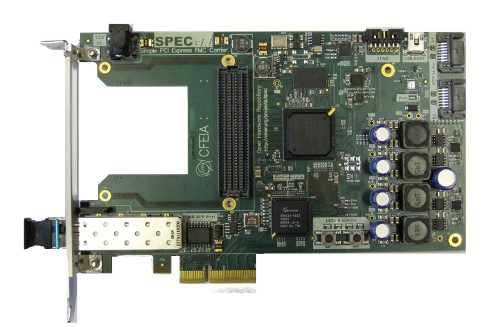
\includegraphics[width=70mm]{img/WEPGF089f5}
   \caption{Commercially available SPEC card.}
   \label{SPEC}
\end{figure}

The SPEC card hardware specification, availability of design sources on OHR along with its low-cost commercial availability made it an attractive solution as the new hardware platform for upgrading Diamond FA Archiver. It was also our aim to interact and build experience with OHW initiative as a user.

\section{FA Archiver on SPEC Card}

The initial challenges with the OHW repository at the start of our project were:

\begin{itemize}
\setlength\itemsep{0em}
\item Understanding our way around the OHR since hardware, firmware and software projects for the SPEC card are maintained in separate repositories.
\item Finding details of the components and features of the SPEC card due to lack of a Hardware User Guide.
\end{itemize}

By studying the open-source board schematics and reference firmware design available on the repository, we were able to identify the modifications to be taken towards implementing the FA Archiver on the SPEC card.

\subsection{PCI Express Interface}
The Spartan-6 FPGA on the SPEC card doesn't have an embedded PCIe IP block unlike the Virtex-5 FPGA on the ML555 board. As a result, an external PCIe bridge, Gennum GN4124, is used to handle the host communication on the SPEC card. This hardware difference required a completed re-implementation of FA Archiver's existing PCIe and interrupt interface logic so that the communication is achieved by using the external bridge's local interface rather than the embedded Xilinx IP block.

\subsection{Clocking Resources}
The SPEC card was design specifically targeting the White Rabbit project, therefore the clocking resources around the FPGA was built on WR requirements which wouldn't suit the DCC. To achieve the required clocking frequency of 106.25MHz for DCC, an external on-board programmable oscillator is used. This was achieved by modifying the DCC firmware to route the clock using on-chip global buffers rather than dedicated MGT clocking pins. This scheme introduces unwanted jitter on the clock, but since MGTs on the FPGA are qualified up to 6.8 Gbps, its effect at the DDC line rate of 2.12 Gbps does not create any unwanted bit errors rates. This modification on the clock routing created additional conflicts for the main FPGA system clock input. This was solved by eliminating the use of the dedicated system clock inputs, and using the PCIe bridge's local clock as the FPGA system clock.

\subsection{On-Chip Communication}
The reference firmware design for the SPEC card uses the Wishbone System-on-Chip (SoC) bus for interconnecting IP cores. The FA Archiver design uses ARM's Advanced Microcontroller Bus Architecture (AMBA) which is the adopted solution for interconnecting Xilinx IPs. Towards achieving the maximum re-use of reference design IPs, FA Archiver's Target and DMA Control Logic design blocks handling the status and control registers for operating the board were also modified to adopt the Wishbone bus.

The resulting FPGA design architecture for the FA Archiver on the SPEC card is shown in 
Fig~\ref{SPECS}.

\begin{figure}[t!]
   \centering
   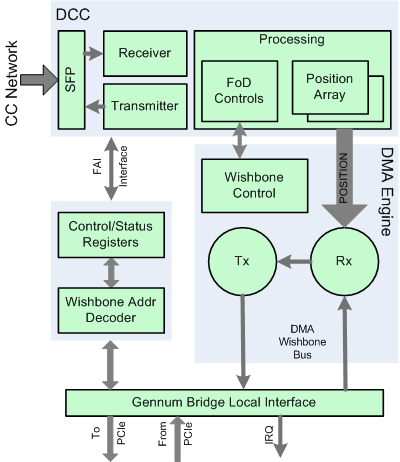
\includegraphics[width=70mm]{img/WEPGF089f6}
   \caption{Architecture of the FA sniffer FPGA on SPEC card. The design interfaces to an external PCIe bridge using the parallel local interface.}
   \label{SPECS}
\end{figure}

\subsection{Software}
The only software modification was in the device driver to detect and identify the card installed (ML555 or SPEC), since the SPEC card's PCIe chip has to be initialised before bringing the interface up. The archiver processing software and client tools as explained in ~\cite{ARCHIVER} didn't require any modifications keeping the back-compatibility.

\section{Summary}
\balance
The motivation for the new FA Archiver interface has been to address obsolescence of the existing PCIe platform, and move to an open platform for continuing support in the community. We took this opportunity to get familiar with Open Hardware initiative, and build experience with the inner workings of the repository. The upgrade project has been successfully completed with initial challenges due to learning stages involved. The new FA Archiver has been running at ALBA for the last year, and will be evaluated by LNLS with DCC running at an increased line rate of 5 Gbps.

\iffalse  % only for "biblatex"
	\newpage
	\printbibliography

% "biblatex" is not used, go the "manual" way
\else

%\begin{thebibliography}{9}   % Use for  1-9  references
\begin{thebibliography}{9} % Use for 10-99 references

\bibitem{ARCHIVER}
M.G. Abbott, G. Rehm, I. Uzun, {\it A New Fast Data Logger and Viewer at Diamond: the FA Archiver }, Proc. of ICALEPCS'2009, Grenoble (France).

\bibitem{FOFB}
M.T.Heron, et al., {\it Diamond Light Source Electron Beam Position Feedback: Design, Realization and Performance}, Proc. of ICALEPCS'2009, Kobe (Japan). 

\bibitem{DCC}
I. Uzun, et al., {\it Initial Design of the Fast Orbit Feedback System for Diamond Light Source}, 
Proc. of ICALEPCS'2005, Geneva (Switzerland). 

\bibitem{ML555}
Xilinx, {\it Virtex-5 LXT ML555 FPGA Development Kit for PCI Express}, \url{http://www.xilinx.com/products/boards-and-kits/HW-V5-ML555-G.htm}

\bibitem{OHW}
CERN, {\it Open Hardware At CERN-Knowledge Transfer}, \url{http://knowledgetransfer.web.cern.ch/files/OH-web.pdf}.

\bibitem{OHL}
CERN, {\it Open Hardware License}, \url{www.ohwr.org/cernohl}.

\end{thebibliography}
\vspace{10mm}
\fi

\end{document}